% ============================================================
% Template de TCC (Artigo Científico) — Faculdade UCL
% Versão simplificada: documentclass "article" padrão, fonte
% Computer Modern (pdfLaTeX), sem formatação ABNT customizada
% (sem capa separada, títulos de seção em maiúsculas simples,
% autores centralizados com notas de rodapé numeradas, legendas
% de figura no padrão default do LaTeX ("Figure")).
%
% Compile com pdfLaTeX (não depende de fontspec/XeLaTeX).
% ============================================================
\documentclass[12pt,a4paper]{article}

\usepackage[a4paper,margin=2.5cm]{geometry}
\usepackage{graphicx}
\usepackage{array}
\usepackage{xcolor}

\setlength{\parindent}{0pt}
\setlength{\parskip}{0.8em}

% ---------- Numeração de página no canto superior direito ----------
\makeatletter
\def\ps@ucl{%
  \def\@oddhead{\hfil\normalfont\thepage}%
  \def\@evenhead{\hfil\normalfont\thepage}%
  \def\@oddfoot{}%
  \def\@evenfoot{}%
}
\makeatother
\pagestyle{ucl}

\begin{document}

% ============================================================
% PÁGINA 1 — cabeçalho, título, autores, resumo
% ============================================================
\thispagestyle{ucl}

\begin{center}
    
\includegraphics[width=3.6cm]{figuras/logo_ucl.png}\\[1em]

    Trabalho de Conclusão de Curso de Engenharia da Computação\\[0.8em]

    \textbf{\MakeUppercase{Protótipo para detecção, localização e seleção automática de ação por sensoriamento}:}\\
    \MakeUppercase{Modelo de dados}\\[0.8em]

    \textbf{\itshape Prototype for automatic action detection, localization and selection through sensing:}\\
    \itshape Data model\\[1.2em]
\end{center}

\begin{center}
    Gabriel Vasconcellos de Morais\footnote{Graduando(a) em Engenharia da Computação pela Faculdade do Centro Leste -- UCL. E-\textit{mail}: gabrielmorais@ucl.br}\\
    Matheus Emanoel Gomes Souza\footnote{Graduando(a) em Engenharia da Computação pela Faculdade do Centro Leste -- UCL. E-\textit{mail}: matheusemanoel@ucl.br}\\
    Anker Douglas Loss\footnote{Orientador(a). Mestre em xxx pela xxx. E-\textit{mail}: anker@ucl.br}
\end{center}

\begin{center}
    \textbf{RESUMO}
\end{center}

\noindent A construção de protótipos de sensoriamento com hardware acessível é um recurso
didático relevante em Engenharia da Computação, por permitir explorar de forma prática conceitos
de aquisição de dados. Integrar sensoriamento de baixo custo, processamento em tempo real e
seleção automática de resposta em um único protótipo exige lidar com comunicação entre hardware e
software e tratamento de leituras ruidosas. Este trabalho tem como objetivo demonstrar a
viabilidade de um sistema de detecção, localização e seleção automática de ação construído
inteiramente com componentes acessíveis, em vez de hardware industrial. O protótipo resultante,
denominado RadarTorres, converte leituras de ângulo e distância em posição cartesiana, exibindo-as
em tempo real em um radar circular, seleciona automaticamente, entre torres candidatas posicionadas
ao redor da base, a mais adequada para responder a cada alvo, e registra em auditoria toda ação
executada. O processamento e a tomada de decisão são concentrados em uma aplicação desktop, com
arquitetura pensada para permitir evolução futura sem exigir hardware adicional. Os requisitos do sistema foram levantados por engenharia reversa diretamente
do código-fonte já implementado. Discutem-se, por fim, as limitações
inerentes à abordagem de baixo custo adotada.

\noindent\textbf{Palavras-chave}: Sensoriamento de baixo custo; Detecção e rastreamento de alvos; Seleção automática de ação; Arduino; Protótipo.

\begin{center}
    \textbf{ABSTRACT}
\end{center}

\noindent This work describes the RadarTorres prototype, a system for automatic action
detection, localization and selection through sensing, developed as a Final Course Project in
Computer Engineering. The prototype integrates sensors to identify objects in a monitored
environment, register their position and allow manual or automatic activation of response
devices. This work details the application's data model: persistence is currently implemented
through CSV files organized per operating-system user, covering six tables -- users, detected
objects, executed actions, mode changes, user preferences and help tickets --, each accessed
through a dedicated repository interface. This choice, documented in the project's technical
records, keeps the system simple at this stage while explicitly signaling the intent to migrate
to a relational database in the future. The current table structure, its relationships (by
login, without real foreign keys) and the proposed model for the SQL migration are described,
in which textual references would be replaced by proper foreign keys, without requiring changes
to the application's ViewModel or Service layers, since they depend only on the repository
interfaces. Results indicate that the interface-based architecture enables this migration
incrementally and with low risk.

\noindent\textbf{Keywords}: Sensing; Data model; Persistence; SQL migration; Prototype.

\clearpage

% ============================================================
% 1 INTRODUÇÃO
% ============================================================
\section{Introdução}

Sistemas automáticos de detecção e resposta a alvos exigem, além de identificar um estímulo,
rastrear com precisão sua posição e aplicar regras de decisão que evitem respostas indevidas --
tarefas comumente resolvidas com sensores de radar ou LIDAR, de custo elevado. Como alternativa a
esse tipo de equipamento, este trabalho adota técnicas de visão computacional, aliadas a hardware
acessível, como parte central da arquitetura do protótipo. Protótipos didáticos construídos dessa
forma desempenham papel importante nesse processo, por permitirem que esses conceitos sejam
explorados de forma prática e replicável em laboratório, reproduzindo os princípios de
sensoriamento, rastreamento e decisão presentes em sistemas mais sofisticados.

% ============================================================
% 2 DESENVOLVIMENTO
% ============================================================
\section{Desenvolvimento}

\subsection{Fundamentação teórica}

Revisão bibliográfica sobre o assunto, com a devida citação das fontes,
por exemplo (SOBRENOME, 2024) ou conforme Sobrenome (2024).

\subsubsection{Sensoriamento de baixo custo e fusão de sensores}

Sensores ultrassônicos medem distância com baixo custo, mas não distinguem o tipo do
obstáculo; câmeras fornecem informação semântica, mas dependem de iluminação e de maior poder
de processamento. A fusão das duas modalidades aproveita essa complementaridade (MAJONI et al.,
2025).

\subsubsection{Seleção automática de ação (TEWA/WTA)}

A escolha do atuador mais adequado a cada alvo é tratada na literatura como um problema de
atribuição de recursos. O RadarTorres adota uma abordagem simples, por proximidade, aplicada
alvo a alvo, com propósito exclusivamente demonstrativo.

\subsection{Procedimentos metodológicos}

O percurso metodológico deste trabalho não seguiu o fluxo tradicional de especificação prévia
seguida de implementação: o protótipo RadarTorres já existia, em desenvolvimento incremental,
antes do levantamento formal de requisitos. Optou-se, portanto, por uma abordagem de engenharia
reversa documental, na qual os requisitos funcionais e não funcionais foram extraídos diretamente
do código-fonte já implementado (\texttt{src/RadarTorres.App/}), do firmware de simulação
(\texttt{Arduino/ArduinoSimulation.ino}) e da documentação técnica já produzida ao longo do
projeto, em vez de definidos a priori em um documento de especificação anterior à codificação.

Esse levantamento resultou em 25 requisitos funcionais (RF01--RF25) e 20 requisitos não
funcionais (RNF01--RNF20), classificados segundo dois critérios objetivos: a \textbf{prioridade},
atribuída conforme a criticidade de cada requisito para a operação central do sistema
(comunicação serial, rastreamento, seleção de torre, modos de operação e segurança recebem
prioridade Alta; suporte administrativo e ferramental, Média; conveniências de interface, Baixa);
e o \textbf{status}, que reflete o estado real de implementação constatado no código no momento do
levantamento -- Implementado, Parcial ou Planejado --, e não a intenção original de projeto. Cada
requisito foi, além disso, rastreado até a classe ou método do código-fonte que o realiza, registro
mantido em uma matriz de rastreabilidade dedicada, de modo que qualquer afirmação sobre o grau de
implementação do protótipo possa ser verificada diretamente no código. Divergências encontradas
entre o comportamento observado no código e a nomenclatura ou fluxo originalmente esperado também
foram registradas explicitamente, em vez de omitidas ou corrigidas silenciosamente na
documentação.

A validação funcional do protótipo, por sua vez, não foi realizada sobre o hardware físico, ainda
não montado: o sistema conta com um modo de simulação embutido na própria aplicação, que gera
leituras sintéticas de ângulo e distância no mesmo formato produzido pelo Arduino, permitindo
exercitar de ponta a ponta o rastreamento de alvos, a seleção automática de torre e as regras de
zona morta sem depender de uma porta serial conectada. Esse modo de simulação foi o meio primário
usado para observar o comportamento do sistema durante este trabalho, o que impõe um limite claro
ao escopo dos resultados relatados: eles atestam a corretude da lógica de decisão implementada em
software, mas não substituem uma validação de campo com sensores e torres físicas, deixada como
trabalho futuro.

\subsection{Diagrama de pacotes}

A organização interna da aplicação desktop foi documentada por meio de um diagrama de pacotes,
diagrama estrutural da UML que representa a divisão lógica do sistema em pacotes e as
dependências existentes entre eles, sem detalhar atributos ou métodos das classes neles contidas.
No RadarTorres, cada pacote corresponde a um \textit{namespace} do projeto
\texttt{RadarTorres.App}, coincidente com uma pasta do código-fonte, e o diagrama foi obtido
diretamente do código da \textit{branch} principal do repositório: cada seta representa ao menos
uma diretiva \texttt{using RadarTorres.App.*} (ou uma referência \texttt{clr-namespace} em XAML)
presente nos arquivos do pacote de origem, de modo que o diagrama descreve a estrutura efetivamente
implementada, e não apenas a pretendida.

\begin{figure}[htbp]
  \centering
  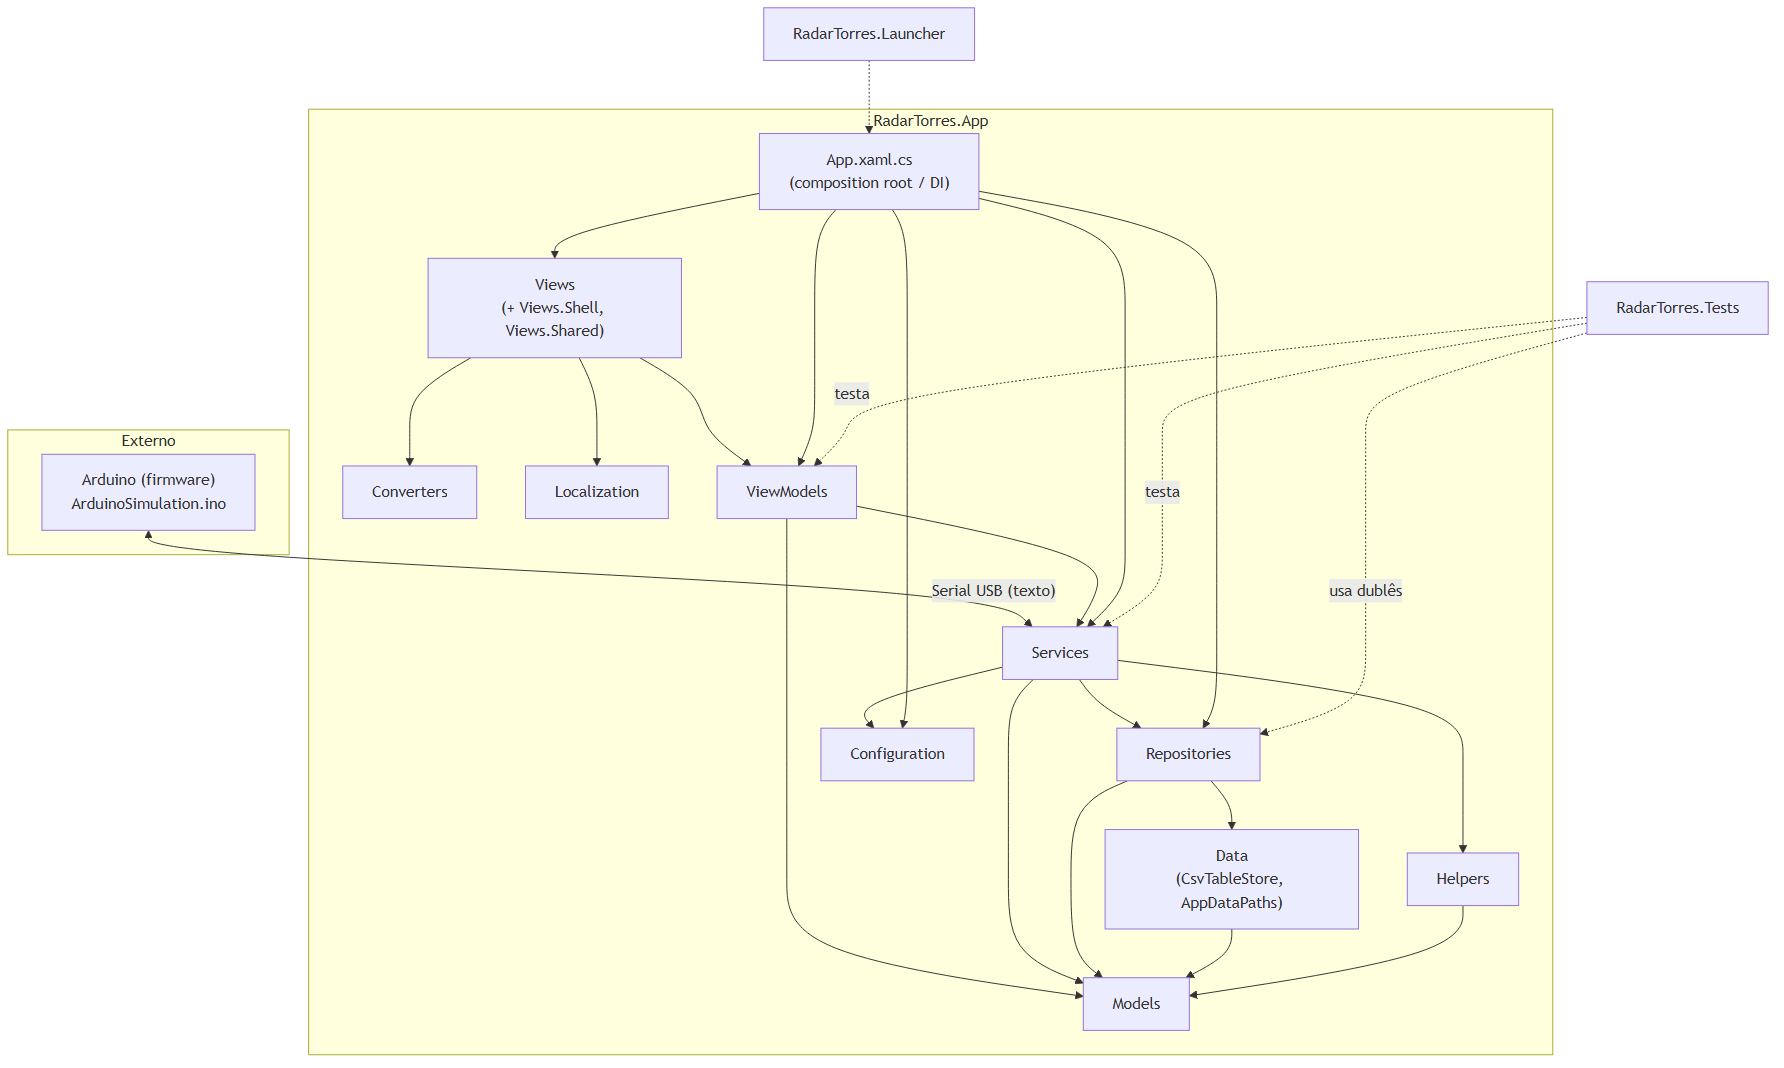
\includegraphics[width=\textwidth]{figuras/Diagrama_de_Pacotes.png}
  \caption{Diagrama de pacotes do RadarTorres. Setas em vermelho indicam dependências que formam
  ciclos (dos autores).}
\end{figure}

O fluxo principal de dependências segue a organização do padrão MVVM, de cima para baixo: Views
$\rightarrow$ ViewModels $\rightarrow$ Services $\rightarrow$ Repositories $\rightarrow$ Data
$\rightarrow$ Models. O pacote Models ocupa a posição mais estável do sistema -- todos os demais
dependem dele e ele não depende de nenhum outro --, o que é desejável para as entidades de
domínio, e a separação entre as interfaces de Repositories e a implementação em CSV do pacote Data
é o que viabiliza a futura migração para um banco relacional sem alterar ViewModels ou Services. A
construção do diagrama a partir do código revelou, também, três dependências que formam ciclos
entre pacotes -- destacadas em vermelho na figura --: o \texttt{NavigationService} importa
\textit{namespaces} de Views para instanciar telas (Services $\rightarrow$ Views), e o
\texttt{DataSeeder}, responsável pela carga inicial de dados, depende de Repositories e de
Services, enquanto esses mesmos pacotes dependem de Data. Esses ciclos não impedem o funcionamento
da aplicação, pois todos os pacotes pertencem ao mesmo \textit{assembly}, mas aumentam o
acoplamento e dificultam testes isolados e futuras separações em projetos distintos.

\subsection{Modelo de dados}

A persistência do RadarTorres foi igualmente documentada por meio de um levantamento do modelo de
dados diretamente a partir do código-fonte já implementado. O protótipo não utiliza, no estágio
atual, um sistema gerenciador de banco de dados relacional: seis entidades -- usuários, objetos
detectados, ações realizadas, trocas de modo de operação, preferências de usuário e chamados de
suporte -- são persistidas localmente em arquivos CSV, um por tabela, cada uma acessada
exclusivamente por uma interface de repositório dedicada, o que isola as camadas de ViewModel e
Service do formato de armazenamento.

\begin{figure}[htbp]
  \centering
  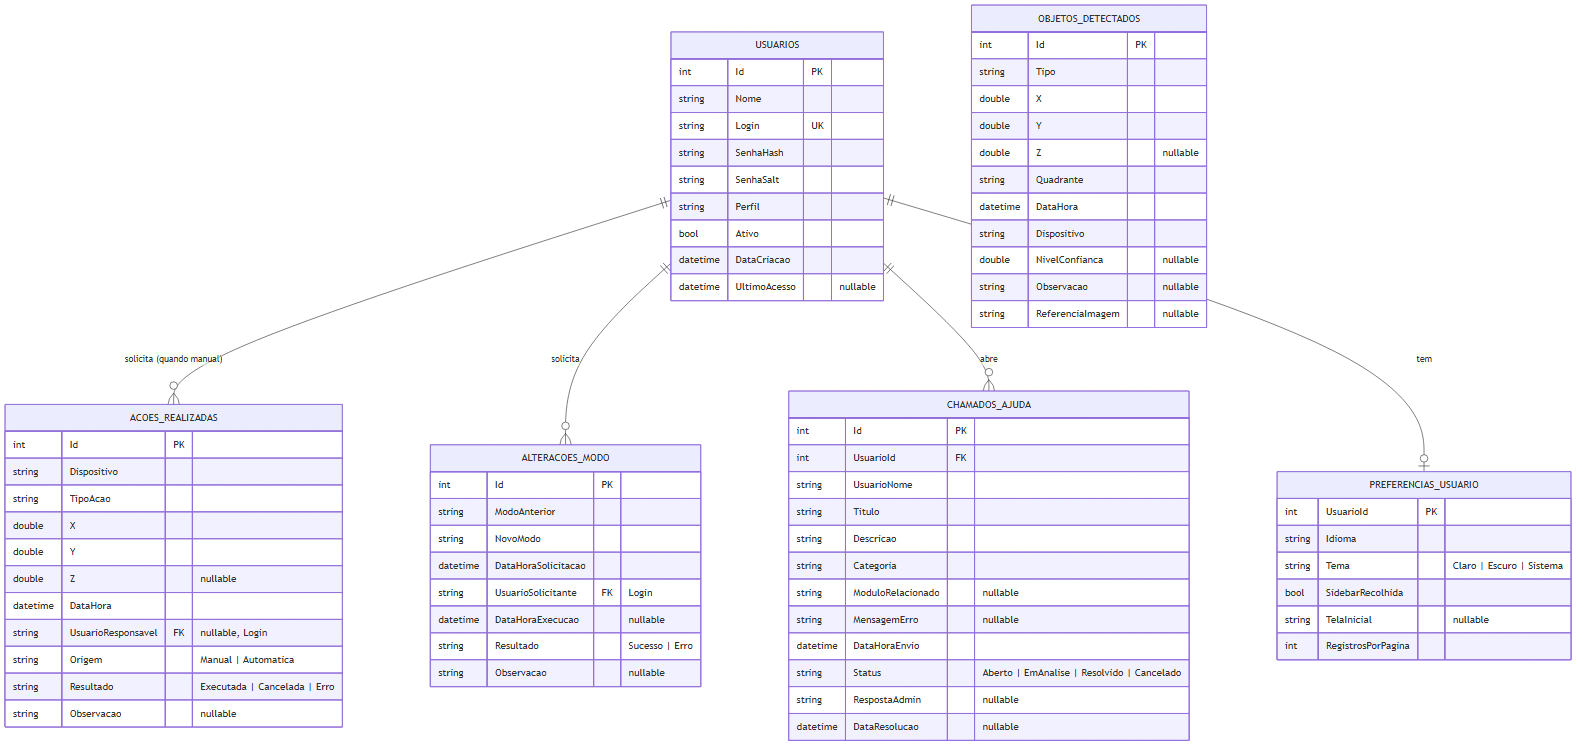
\includegraphics[width=\textwidth]{figuras/DER_Atual.png}
  \caption{Modelo de dados atual (persistência em CSV) -- diagrama entidade-relacionamento
  levantado a partir do código-fonte do projeto (dos autores).}
\end{figure}

\texttt{Usuario} se relaciona 1:1 com \texttt{PreferenciasUsuario} e 1:N com
\texttt{AcaoRealizada} e \texttt{ModoAtualTorre} -- nesses dois últimos casos por \textbf{login}
(texto), sem chave estrangeira real -- e com \texttt{ChamadoAjuda}, por identificador numérico.
\texttt{ObjetoDetectado} não possui nenhum vínculo persistido com as demais entidades, sendo
registrado de forma independente. Como proposta de evolução, foi elaborado um modelo relacional
equivalente, no qual as referências textuais por login seriam substituídas por chaves estrangeiras
íntegras por identificador numérico, com integridade garantida pelo próprio SGBD, permitindo migrar
a persistência de CSV/JSON para SQL sem exigir alterações nas camadas de ViewModel ou Service, já
isoladas do formato de armazenamento por meio das interfaces de repositório.

\begin{figure}[htbp]
  \centering
  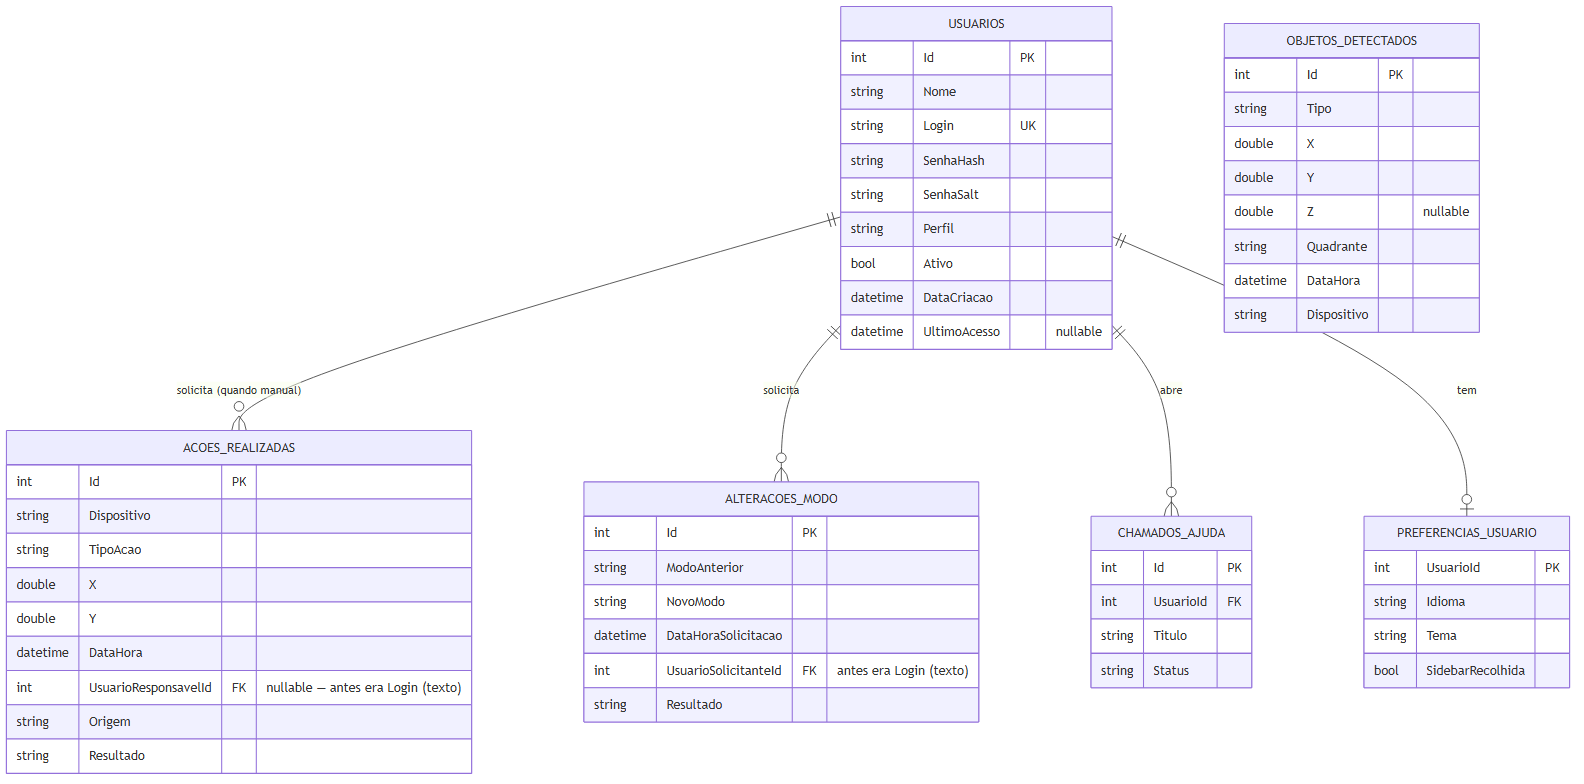
\includegraphics[width=\textwidth]{figuras/DER_Proposto.png}
  \caption{Modelo relacional proposto para a migração futura de persistência, de CSV/JSON para SQL
  (dos autores).}
\end{figure}

\end{document}
